% Appendix A

\chapter{Controlador \textsc{PID} para motores de \textsc{DC}} % Main appendix title

\label{AppendixA} % For referencing this appendix elsewhere, use \ref{AppendixA}

\section{Controlador \textsc{PID}}

Fundamentalmente, los controladores \textsc{PID} est\'an compuestos de tres
acciones de control b\'asicas. Estas son de simple implementaci\'on y
proporcionan un buen rendimiento. Los proceso de ajuste de las ganancias de los controladores 
PID puede ser complejo porque es iterativo: primero, es necesario sintonizar el modo 
\emph{Proporcional}, luego el \emph{Integral}, y luego agregue el modo
\emph{Derivado} para estabilizar el sobreimpulso, luego agrega más
\emph{Proporcional}, y así sucesivamente. El PID controlador tiene la siguiente forma en el dominio de tiempo:
\begin{figure}[th]
    \centering
    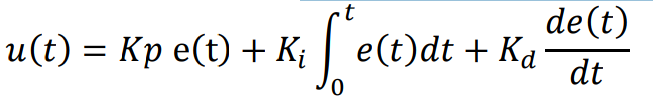
\includegraphics[width=.7\textwidth]{Figures/eq1.png}
    \label{fig:eqpid}
\end{figure}
Donde e $(t)$ es el error del sistema (diferencia entre
entrada de referencia y la salida del sistema), $u(t)$ el control
variable, $Kp$ la ganancia proporcional, $Ki$
 la ganancia integral,
y $Kd$
 es la ganancia derivada. Cada coeficiente del \textsc{PID}
controlador agrega algunas caracter\'isticas especiales a la salida
respuesta del sistema Debido a esto, elegir el
par\'ametros correctos se convierte en una decisi\'on crucial para poner
en pr\'actica este controlador. Los efectos de estos
par\'ametros en la respuesta de salida del sistema son
que se muestra en la Tabla (2).
 Un controlador PID no "conoce" la salida correcta
para llevar el sistema al punto establecido mueve la salida
en la direcci\'on que deber\'ia mover el proceso hacia
el punto de ajuste y necesita tener retroalimentaci\'on (mediciones)
actuar.

La funci\'on objetivo principal que se selecciona para ser
minimizado ser\'a considerado en este estudio:

\begin{figure}[th]
    \centering
    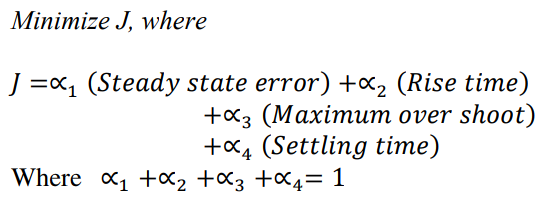
\includegraphics[width=.7\textwidth]{Figures/demo1.png}
    \label{fig:demo}
\end{figure}

Esta funci\'on objetivo $J$ proporciona un punto de funcionamiento que
en general es una transacc\'on de los cuatro t\'erminos ponderados del
Controlador \textsc{PID} seg\'un los valores de los pesos $\alpha_1$,
$\alpha_2$, $\alpha_3$ y $\alpha_4$, donde $\alpha_1$, $\alpha_2$, $\alpha_3$ y
$\alpha_4$ est\'an ponderando
factores de los cuatro t\'erminos clave. \parencite{pid}
